\documentclass{article}
\usepackage[T2A]{fontenc}
\usepackage[utf8]{inputenc}
\usepackage[russian,english]{babel}
\usepackage{listings}
\usepackage{indentfirst}
\usepackage{graphicx}
\usepackage{array}
\usepackage{wrapfig}
\usepackage{multirow}
\usepackage{tabularx}
\graphicspath{ {./images/} }
\usepackage{geometry}
\geometry{verbose,a4paper,tmargin=2cm, bmargin=2cm, lmargin=2.5cm, rmargin=1.5cm}

\usepackage{xcolor}

\definecolor{codegreen}{rgb}{0,0.6,0}
\definecolor{codegray}{rgb}{0.5,0.5,0.5}
\definecolor{codepurple}{rgb}{0.58,0,0.82}
\definecolor{backcolour}{rgb}{0.95,0.95,0.92}

\lstdefinestyle{mystyle}{
    backgroundcolor=\color{backcolour},   
    commentstyle=\color{codegreen},
    keywordstyle=\color{magenta},
    numberstyle=\tiny\color{codegray},
    stringstyle=\color{codepurple},
    basicstyle=\ttfamily\footnotesize,
    breakatwhitespace=false,         
    breaklines=true,                 
    captionpos=b,                    
    keepspaces=true,                 
    numbers=left,                    
    numbersep=5pt,                  
    showspaces=false,                
    showstringspaces=false,
    showtabs=false,                  
    tabsize=2
}

\lstset{
language = C++,
style = mystyle,
extendedchars=\true}



\title{Параллельная реализация алгоритмов численного интегрирования на языке С++ с использованием OpenMP}
\author{Оришин И.C.}
\date{Май 2020}


\begin{document}

\maketitle
\newpage
\section{Первые приготовления}
\subsection{Используемые расширения}
Для успешной реализации методов численного интегрирования на языке С++. Нам понадобятся следующие расширения:
\begin{itemize}
  \item stdio.h – стандартная библиотека языка C;
  \item iostream – стандартная библиотека языка C++;
  \item iomanip – стандартная библиотека языка C++
  \item math.h – математический модуль языка С;
  \item omp.h – библиотека стандарта openMP;
  \item string – библиотека STL;
  \item chrono – библиотека манипуляций со временем;
  \item random – библиотека ГСЧ;
\end{itemize}

Для последних двух библиотек введу некоторые пояснения. Библиотека chrono
будет использоваться для оценки времени работы программы. Она обеспечивает более
высокую точность измерений по сравнению с модулем time. Библиотеку random будем
использовать для упрощения генерации случайных чисел, а также для обеспечения более "случайной" работы генератора. 
Не забудем указать, что будем использовать пространство имён std. Первые приготовления завершены.
\begin{lstlisting}
#include <stdio.h>
#include <iostream>
#include <math.h>
#include <omp.h>
#include <string>
#include <chrono>
#include <random>
#include <iomanip> 

using namespace std;

int main(int argc, char* argv[]){
    return 0;
}
\end{lstlisting}
\subsection{Генератор случайных чисел}
В процессе работы у нас возникнет необходимость в генерации случайных вещественных чисел. Для сокращения времени выполнения работы программы генератора, будем генерировать числа сразу скопом, причем параллельно. Для этого каждый поток будет генерировать своё случайное число и сразу записывать его в массив. Я предлагаю реализовать это следующим образом:
\begin{lstlisting}
void randdouble(double min, double max, double *arr, int n){
    random_device rd;
    mt19937 gen(rd());
    uniform_real_distribution<> dis(min, max);
    #pragma omp parallel for
    for (int i = 0; i < n; i++){
        arr[i] = dis(gen);
    }
}
\end{lstlisting}
Данная функция на входе "кушает" следующие параметры: 
\begin{itemize}
    \item min - ограничение снизу интервала случайных чисел;
    \item max - ограничение сверху интервала случайных чисел;
    \item *arr - указатель на массив сгенерированных случайных чисел;
    \item n - размер массива случайных чисел.
\end{itemize}
Первые две строки определяют устройство генерации(rd) и функцию генерации(gen)
\textbf{uniform\char`_real\char`_distribution<>} тип возвращаемого объекта. В данном случае
получим действительное случайное распределение. dis(min,max) - сам объект В цикле каждому элементу массива присвоим сгенерированный элемент с помощью \textbf{dis(gen)}. Распараллелим цикл при помощи прагмы \textbf{omp parallel for}.
Пример использования функции:

\begin{lstlisting}
int a = 0; b = 10; // Интервал генерации [0;10]
int n = 10; // Размер массива
double *x = new double[n];
randdouble(a, b, x, n);
\end{lstlisting}
\subsection{Определение времени работы программы}
Для определения времени работы какой-либо функции целесообразно использовать
библиотеку chrono. Алгоритм работы максимально простой:
\begin{enumerate}
    \item Получить текущее время
    \item Выполнить операцию
    \item Получить текущее время
    \item Посчитать разницу между временами до и после
\end{enumerate}
Для успешной реализации нам понадобятся две функции из библиотеки chrono:
\begin{itemize}
    \item \texttt{chrono::steady\char`_clock::now();} - получает текущее время
    \item \texttt{chrono::duration\char`_cast<std::chrono::duration<double>>} - считает разницу между двумя временами
\end{itemize}
Пусть startTime - начальное время, endTime - конечное, runTime - время исполнения операции. В качестве типа будем использовать тип auto. Тогда:
\begin{lstlisting}
auto startTime = chrono::steady_clock::now();
foo() // Целевая функция
auto endTime = chrono::steady_clock::now();
auto runTime = chrono::duration_cast<std::chrono::duration<double>>(endTime-startTime);
cout<<"Время работы целевой функции"<<runTime<<endl;
\end{lstlisting}
\subsection{Передача функции в функцию}
Для того, чтобы избежать дублирование кода в некоторых моментах, я использовал
механизм передачи функции в функцию. Для начала я определил новый тип с 
помощью typedef double(*function)(double, double). Эта строчка означает, что 
теперь у меня есть объект - функция с двумя параметрами. И теперь чтобы передать функцию foo в функцию bar как параметр мне нужно всего ничего:
\begin{lstlisting}
typedef double(*function)(double, double)

double foo(double x,double y){...}
double bar(function f){...}

int main(int argc, char* argv[]){
    bar(&foo);
}
\end{lstlisting}
\subsection{Подготовка функций}
Для реализации алгоритмов я выбрал следующие функции и их пределы интегрирования:
\begin{center}
$$f(x) = \frac{x^2 + sin (0.48 * (x + 2))}{\exp(x^2)+0,38} $$
$x \in [a,b]$$

$$g(x,y) = \frac{(x+y)^2}{x}$$ 
$$x \in [a,b]$$
$$y \in [x,\frac{x}{2}] $

\end{center}
Нам требуется описать их согласно нашему шаблону. Дело в том, что шаблонная функция
принимает два аргумента, а в функцию f требуется всего лишь один. Сделаем хитрый трюк
добавим в параметр функции аргумент-заглушку arg. Он будет передаваться в функцию, но использоваться в ней не будет. Точнее не будет использоваться только в одномерных методах. Забегая вперед, скажу, что это очень важно для двумерных методов и когда мы до них дойдем я всё объясню. Соответственно, передающийся аргумент-заглушка может быть любым. Какая разница что там передалось, если это не используется? Аргументами функции являются границы интегрирования. Все же понимают, что численно интегрировать можно только определённый интеграл. 
Напишем функцию f:
\begin{lstlisting}
double f(double arg, double x){
  return (pow (x, 2) + sin (0.48 * (x + 2))) / (exp (pow (x, 2)) + 0.38);
}
\end{lstlisting}
Наша функция соответствует следующему интегралу:
\begin{center}
$$\int\limits_a^b \frac{x^2 + sin (0.48 * (x + 2))}{\exp(x^2)+0,38}\,dx$$
\end{center}
С функцией g всё проще. Она и так принимает два аргумента. Поэтому напишем её как есть:
\begin{lstlisting}
double g(double x, double y){
    return pow(x+y,2)/x;
}
\end{lstlisting}
Но, к сожалению, данный вариант работать не будет. Точнее будет, но не так как хотелось бы. Дело в том, что у двойного интеграла границ интегрирования не две а 4.
Вот так:
$$\int\limits_a^b \int\limits_x^\frac{x}{2} \frac{(x+y)^2}{x}\,dxdy$$
Это означает, что продолжать считать интеграл нам нужно только тогда, когда соблюдены условия внутренних границ интегрирования:
\begin{lstlisting}
double g(double x, double y){
    if  ((y < x) and (y > x/2)){
        return pow(x+y,2)/x;
    } else 
    return 0;
}
\end{lstlisting}
Отлично. Теперь это будет работать. Данный код мне показался немного страшным, поэтому я решил добавить немного синтаксического сахара в виде тернарного оператора. Чтобы понять суть работы этого оператора достаточно посмотреть на верхний и нижний код. Они идентичны.
\begin{lstlisting}
double g(double x, double y){
    return  ((y < x) and (y > x/2)) ? pow(x+y,2)/x : 0;
}
\end{lstlisting}
\subsection{Соберём знания в кучу}
Собрав всё в кучу получаем следующий код.
\begin{lstlisting}
#include <stdio.h>
#include <iostream>
#include <math.h>
#include <omp.h>
#include <string>
#include <chrono>
#include <random>
#include <iomanip> 

typedef double(*function)(double, double);

using namespace std;

void randdouble(double min, double max, double *arr, int n){
    random_device rd;
    mt19937 gen(rd());
    uniform_real_distribution<> dis(min, max);
    #pragma omp parallel for
    for (int i = 0; i < n; i++){
        arr[i] = dis(gen);
    }
}

double g(double x, double y){
    return  ((y < x) and (y > x/2)) ? pow(x+y,2)/x : 0;
}

double f(double arg, double x){
  return (pow (x, 2) + sin (0.48 * (x + 2))) / (exp (pow (x, 2)) + 0.38);
}

int main(int argc, char* argv[]){
return 0;
}
\end{lstlisting}
Знания о том, как считать время работы программы и передаче функции в функцию нам понадобятся позже. Теперь мы готовы писать одномерные численные методы.
\section{Реализация методов численного интегрирования для одномерных функций}
\subsection{Методы прямоугольников}
Реализацию одномерных методов начнём с простых и пойдём по нарастающей. Первый в списке у нас пойдет метод левых прямоугольников. Его суть довольно проста. Нужно
разбить область интегрирования на прямоугольники с определенным шагом. Чем больше шаг, тем больше прямоугольников получится. Метод левых прямоугольников подразумевает разбиение так, чтобы коснуться целевой функции левыми углами, как показано на рисунке 1.
\begin{center}
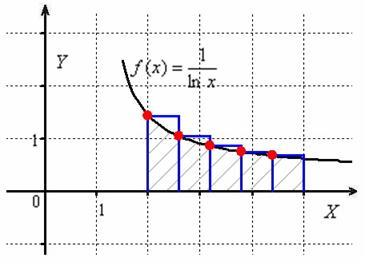
\includegraphics{images/lr.jpg}

Рисунок 1. Метод левых прямоугольников
\end{center}
Затем, требуется посчитать значение в каждой точке и суммировать их. Формул бывает два типа: для одинакового шага на всем промежутке разбиения и для разных шагов. В данной работе я буду пользоваться только формулами для одинакового шага, так называемыми составными формулами для равномерных сеток, поэтому формулы для разных шагов здесь обсуждаться не будут. Формула для равномерной сетки выглядит следующим образом:
$$\int\limits_a^b f(x)dx \approx h\sum_{i=0}^{n-1}f_i = h(f_0,f_1,...,f_{n-1})$$
Шаг сетки h и входное значение $x_i$ рассчитывается как:
$$h = \frac{b-a}{n}; x_i = a+ih,$$
где n - количество разбиений(прямоугольников).
Теперь, когда мы разобрались с формулой нам осталось только написать функцию.
Функция будет принимать на "покушать" следующие аргументы:
\begin{itemize}
    \item f - целевая функция(тип function, который мы заранее определили);
    \item arg - аргумент заглушка, который нас не интересует, так как ни на что не влияет;
    \item a - нижний предел интегрирования;
    \item b - верхний предел интегрирования;
    \item n - количество разбиений.
\end{itemize}
\begin{lstlisting}
double left_rects(function f, double arg, double a, double b, int n){
    double S = 0.0, h = (b-a)/n;
    #pragma omp parallel for reduction(+:S)
    for (int i = 0; i < n - 1; i++) S += f(arg, a + i*h); //arg - заглушка
    return S * h;
}
\end{lstlisting}
В этом коде мы задаем сумму равную 0 и шаг разбиения. Затем пишем цикл предварительно распараллелив его с помощью директивы reduction. Напомню, что директива reduction создает общую для всех потоков переменную S, к которой каждый поток самостоятельно добавляет значение.
Проверить работу функции можно следующим образом:
\begin{lstlisting}
int main(int argc, char* argv[]){
    cout<<left_rects(&f,0,0,10,10);<<endl;
return 0;
}
\end{lstlisting}

Приступим к методу правых прямоугольников. Этот метод отличается от предыдущего лишь тем, что коснуться целевой функции нужно правыми углами прямоугольников, как показано на рисунке 2.
\begin{center}
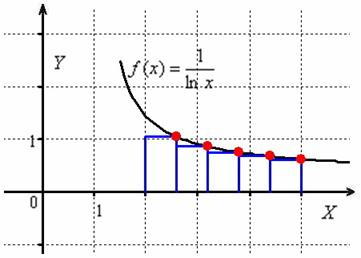
\includegraphics{images/rr.jpg}

Рисунок 2. Метод правых прямоугольников
\end{center}
Соответственно от этого незначительно меняется и формула, параметры шага и входного значения остаются такими же.
$$\int\limits_a^b f(x)dx \approx h\sum_{i=1}^{n}f_i = h(f_1,f_2,...,f_{n})$$
Следовательно мы без труда можем написать этот код, входные значения функции останутся неизменными:
\begin{lstlisting}
double right_rects(function f, double arg, double a, double b, int n){
    double S = 0.0, h = (b-a)/n;
    #pragma omp parallel for reduction(+:S)
    for (int i = 1; i < n; i++) S += f(arg, a + i*h); //arg - заглушка
    return S * h;
}
\end{lstlisting}
Проверить работу функции можно следующим образом:
\begin{lstlisting}
int main(int argc, char* argv[]){
    cout<<right_rects(&f,0,0,10,10);<<endl;
return 0;
}
\end{lstlisting}
Приступим к методу средних прямоугольников. Этот метод отличается от других тем, что
коснутся целевой функции теперь предстоит серединой верхней стороны прямоугольника, как показано на рисунке 3.
\begin{center}
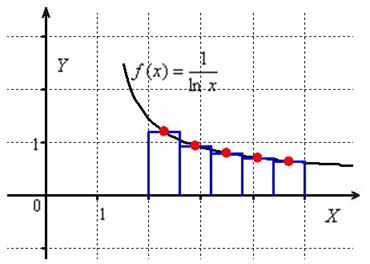
\includegraphics{images/mr.jpg}

Рисунок 3. Метод средних прямоугольников
\end{center}
Формула для расчёта выглядит следующим образом:
$$\int\limits_a^b f(x)dx \approx h(\frac{f_1}{2},\frac{f_2}{2},...,\frac{f_{n-1}}{2})$$
Чтобы понять, почему формула выглядит так, а не иначе, возьмите любую из картинок, озвученных выше методов и попробуйте мысленно сдвинуть прямоугольники влево или вправо в зависимости от варианта так, чтобы красная точка оказалось посередине. Вне зависимости от того, какой вариант вы выбрали, вы увидите, что половина прямоугольника добавится справа или слева, а противоположная половина исчезнет.
Шаг останется такой же, а вот чтобы получить правильное входное значение прибавим к существующему полшага, тем самым сдвинув его на середину.
$$h = \frac{b-a}{n}; x_i = a+ih+\frac{h}{2}$$
Реализуем этот метод, входные параметры не изменятся:
\begin{lstlisting}
double middle_rects(function f, double arg, double a, double b, int n){
    double S = 0.0, h = (b-a)/n;
    #pragma omp parallel for reduction(+:S)
    for (int i = 0; i < n-1; i++) S += f(arg, a + i*h+h/2); //arg - заглушка
    return S * h;
}
\end{lstlisting}
Проверить работу функции можно следующим образом:
\begin{lstlisting}
int main(int argc, char* argv[]){
    cout<<middle_rects(&f,0,0,10,10);<<endl;
return 0;
}
\end{lstlisting}

Все методы прямоугольников готовы, и мы можем насладится результатом:
\begin{lstlisting}
double left_rects(function f, double arg, double a, double b, int n){
    double S = 0.0, h = (b-a)/n;
    #pragma omp parallel for reduction(+:S)
    for (int i = 0; i < n - 1; i++) S += f(arg, a + i*h); //arg - заглушка
    return S * h;
}

double right_rects(function f, double arg, double a, double b, int n){
    double S = 0.0, h = (b-a)/n;
    #pragma omp parallel for reduction(+:S)
    for (int i = 1; i < n; i++) S += f(arg, a + i*h); //arg - заглушка
    return S * h;
}

double middle_rects(function f, double arg, double a, double b, int n){
    double S = 0.0, h = (b-a)/n;
    #pragma omp parallel for reduction(+:S)
    for (int i = 0; i < n-1; i++) S += f(arg, a + i*h+h/2); //arg - заглушка
    return S * h;
}
\end{lstlisting}

Хотя нет, не можем. Посмотрите, мы ведь написали один и тот же код три раза!!! Это никуда не годится! Подумал я и придумал изящное решение этой проблемы. Посмотрите внимательно на места, где есть отличия. Это параметры цикла и шага в методе средних прямоугольников. Я написал следующий код, в котором заменил эти места:
\begin{lstlisting}
double rect_method_x(function f, double arg, double a, double b, int n, int k){
    double S = 0.0, h = (b-a)/n;
    #pragma omp parallel for reduction(+:S)
    for (int i = k%2; i < n - k%3; i++) S += f(arg, a + i*h + (k%5)*h/2);
    return S * h;
}
\end{lstlisting}
Мне пришлось добавить еще один аргумент в функции - k, который и будет определять каким методом действовать функции. Я подобрал три числа, в зависимости от которых, те или иные значения будут превращаться в нужные.
\begin{table}[h!]
\centering
\begin{tabular}{|l|l|l|l|}
\hline
k  & k\%2 & k\%3 & k\%5 \\ \hline
10 & 0    & 1    & 0    \\ \hline
15 & 1    & 0    & 0    \\ \hline
16 & 0    & 1    & 1    \\ \hline
\end{tabular}
\end{table}
\newline
Если вы подставите в новый код k = 10 при методе левых прямоугольников, 15 при правых, 16 при средних, то Вы получите в точности три кода которые выше.
Теперь можно вызвать разные методы следующим образом:
\begin{lstlisting}
int main(int argc, char* argv[]){
    cout<<"Левых"<<rect_method_x(&f,0,0,10,10,10);<<endl;
    cout<<"Правых"<<rect_method_x(&f,0,0,10,10,15);<<endl;
    cout<<"Средних"<<rect_method_x(&f,0,0,10,10,16);<<endl;
return 0;
}
\end{lstlisting}
\subsection{Метод трапеций}
Метод трапеций отличается от методов прямоугольников, очевидно, тем, что вместо прямоугольников мы будем использовать трапеции. Нужно построить трапеции около целевой функции таким образом, чтобы скосы максимально были приближены к ней, как показано на рисунке 4.
\begin{center}
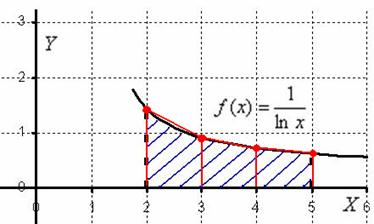
\includegraphics{images/tr.jpg}

Рисунок 4. Метод трапеций
\end{center}
Соответственно, формула для расчета выглядит так:
$$\int\limits_a^b f(x)dx \approx h(\frac{f_0+f_n}{2}+\sum_{i=1}^{n-1} f_i)$$
Параметры шага и входного значения не меняются. Значит нам не составит труда написать эту функцию. Нам нужно всего лишь посчитать полусумму между первым и последним значением функции, затем пройтись по циклу и после умножить полусумму вместе с суммой цикла на шаг. Не забываем при этом параллелить цикл. Входные параметры не меняются, за исключением параметра k - он нам больше не нужен:
\begin{lstlisting}
double trap_method_x(function f, double arg, double a, double b, int n){
    double S = 0.0, step = (b-a)/n;
    double diff = (f(arg, a) + f(arg, b)) / 2; //полусумма
    #pragma omp parallel for reduction(+:S)
    for (int i = 1; i < n - 1; i++) S += f(arg, a + i*step);
    return (diff + S) * step;
}
\end{lstlisting}
Воспользоваться функцией можно следующим образом:
\begin{lstlisting}
int main(int argc, char* argv[]){
    cout<<trap_method_x(&f,0,0,10,10);<<endl;
return 0;
}
\end{lstlisting}
\subsection{Метод Симпсона}
Метод Симпсона является простым, точным и быстрым методом и часто используется для
вычисления интегралов. Формула Симпсона, по которой происходят вычисления с виду кажется страшной:
$$\int\limits_a^b f(x)dx \approx \frac{h}{3}(f(x_0)+2\sum_{i=2}^{n} f_i+4\sum_{i=1}^{n-1} f_i+f(x_n))$$
Но на деле формула не является таковой. Простым языком это звучит так:
\begin{enumerate}
    \item Посчитать значение функции в начале отрезка
    \item Посчитать значение функции в конце отрезка
    \item Посчитать сумму в четных значениях шага и умножить на 2
    \item Посчитать сумму в нечетных значениях шага и умножить на 4
    \item Суммировать всё и умножить на треть шага
\end{enumerate}
Шаг остается таким же, как и в методе прямоугольников.
Википедия предлагает внутри сумм использовать удвоенное значение разбиения, но на деле при достаточно больших n, этим можно пренебречь, чем я воспользовался в процессе кодинга. Входные параметры функции остались неизменными. Проверим написанное согласно нашему алгоритму:
\begin{lstlisting}
double simpson_method_x(function f, double arg, double a, double b, int n){
    //Введем две начальные нулевые суммы и шаг
    double S1 = 0.0, S2 = 0.0, step = (b-a)/n;
    //суммируем значения функции в четных значениях шага
    #pragma omp parallel for reduction(+:S1)
    for (int i = 2; i < n; i+=2) S1 += f(arg, a + i*step);
    //суммируем значения функции в нечетных значениях шага
    #pragma omp parallel for reduction(+:S2)
    for (int i = 1; i < n - 1; i+=2) S2 += f(arg, a + i*step);
    //возвращаем значение функции в начале + в конце + 2 первых суммы + 4 вторых и умножаем на треть шага
    return (f(arg, a) + f(arg, b) + 2*S1 + 4*S2) * step/3.;
}
\end{lstlisting}
Не забываем распараллелить цикл с помощью известной директивы.
Воспользоваться функцией можно следующим образом:
\begin{lstlisting}
int main(int argc, char* argv[]){
    cout<<simpson_method_x(&f,0,0,10,10);<<endl;
    return 0;
}
\end{lstlisting}
\subsection{Метод Ньютона-Котеса (3/8)}
Метод 3/8 очень похож на метод Симпсона, но имеет достаточно непонятную математическую формулу. Поэтому я осмелюсь отойти от принципов фундаментальной математики и как можно проще отобразить эту формулу. Итак:
$$\int\limits_a^b f(x)dx \approx \frac{3}{8}h(f(x_0)+2S_1+3S_2+f(x_n)),$$
где $S_1$ - это сумма в тех значениях шага, которые делятся нацело на три, а $S_2$ - в которых не делятся. Следовательно, закодить формулу можно по следующему алгоритму:
\begin{enumerate}
    \item Посчитать значение функции в начале отрезка
    \item Посчитать значение функции в конце отрезка
    \item Посчитать сумму в тех значениях шага, которые делятся на 3 нацело и умножить её на 2
    \item Посчитать сумму в тех значениях шага, которые не делятся на 3 нацело и умножить её на 3
    \item Суммировать всё и умножить на три восьмых шага
\end{enumerate}
Как обычно, входные значения не меняются значения шага не меняются. Предлагаю мысленно поставить комментарии в код аналогично предыдущему примеру:
\begin{lstlisting}
double nc_method_x(function f, double arg, double a, double b, int n){
    double S1 = 0.0, S2 = 0.0, step = (b-a)/n;
    #pragma omp parallel for reduction(+:S1)
    for (int i = 1; i < n; i++){ if (i % 3 == 0) S1 += f(arg, a + i*step); }
    #pragma omp parallel for reduction(+:S2)
    for (int i = 1; i < n; i++){ if (i % 3 != 0) S2 += f(arg, a + i*step); }
    return 3./8. * (f(arg, a) + f(arg, b) + 2*S1 + 3*S2) * step;
}
\end{lstlisting}
Воспользоваться функцией можно как обычно:
\begin{lstlisting}
int main(int argc, char* argv[]){
    cout<<nc_method_x(&f,0,0,10,10);<<endl;
    return 0;
}
\end{lstlisting}
\subsection{Метод Монте-Карло}
Метод Монте-Карло является довольно необычным и интересным из всех представленных, потому что работает по другому принципу. Суть его состоит в следующем. Допустим у нас есть некоторая функция на плоскости. Возьмем произвольный прямоугольник со сторонами a,b,c,d в котором будем проводить вычисления. Возьмем ручку и натыкаем случайным образом быстро-быстро множество точек. Если мы будем действительно случайно тыкать с закрытыми глазами, например, у нас получится примерно следующая картина:
\begin{center}
    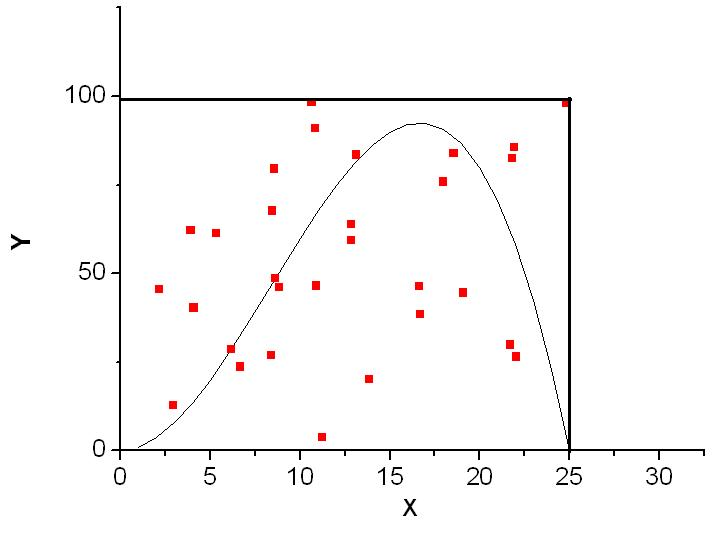
\includegraphics[width=0.8\textwidth]{images/mc.jpg}
    
    Рисунок 5. Метод Монте-Карло
\end{center}
Область ограниченная жирными линиями и осями координат и есть область a,b,c,d.
Теперь Посчитав разницу между сторонами и перемножив, по сути получив площадь прямоугольника, мы должны умножить ее на отношение точек попавших под функцию ко всем точкам. Математически это выглядит так:
$$\int\limits_a^b f(x)dx \approx (b-a)(c-d)\frac{n}{N},$$
где n - количество попавших точек, N - количество всех точек. 
Давайте напишем эту функцию. Тут нам поможет наш генератор случайных чисел, который мы писали в первой главе и следующий алгоритм:
\begin{enumerate}
    \item Генерируем массив точек по x
    \item Генерируем массив точек по y
    \item Проходимся по циклу, проверяя ниже ли находится значение функции в случайной точке x случайной точки y, если да, то увеличиваем счётчик попавших точек
    \item Применяем формулу
\end{enumerate}
Посмотрим на код функции. К входным параметрам теперь добавились границы a,b,c,d - которые являются длинами сторон прямоугольника. Теперь n - это количество точек.
\begin{lstlisting}
double mc_method_x(function f, double arg, double a, double b, double c, double d, int n){
    //выделяем память для массивов, объявляем пустой счётчик
    double *x = new double[n], *y = new double[n]; int in = 0;
    //генерируем массивы с помощью генератора
    randdouble(a, b, x, n);
    randdouble(c, d, y, n);
    #pragma omp parallel for reduction(+:in)
    for (int i = 0; i < n; i++){ if (y[i] < f(arg, x[i])) in++; }
    // сравниваем значение функции со значением в случайной точке
    return (b-a)*(d-c) * in/n;
}
\end{lstlisting}
То, что числа генерируются уже параллельно, держим в голове с первой главы, а также не забываем распараллелить суммирующий цикл.
Воспользоваться функцией можно как обычно:
\begin{lstlisting}
int main(int argc, char* argv[]){
    cout<<mc_method_x(&f,0,0,10,0,10,100);<<endl;
    return 0;
}
\end{lstlisting}
\subsection{Погрешности одномерных методов}
Относительные погрешности считаются также просто, как и всегда. Считается значение
с разбиением n двойным n. Их абсолютная разница и будет являться относительной погрешностью. 
Абсолютные погрешности одномерных методов связаны с одним понятием - максимальное абсолютное значение производной функции. Его суть понятна из названия, но чтобы всем было понятно то алгоритм нахождения "для чайников" следующий:
\begin{enumerate}
    \item Найти требуемую производную функции
    \item Найти её минимум и максимум на промежутке интегрирования
    \item Сравнить, что больше по модулю, то и будет этим числом.
\end{enumerate}
Для данной работы я заранее просчитал все максимальные абсолютные значения производных используемых функций до 4 порядка включительно. В данном пункте я не буду приводить код этих формул, так как это элементарно. Далее я предоставлю формулы погрешностей.
\newline
Погрешность формулы левых и правых прямоугольников
$$E = max_{\{a,b\}} (|{f'(x_i)}|)\frac{(f(b)-f(a))^{2}}{2}$$
Погрешность формулы средних прямоугольников
$$E = max_{\{a,b\}} (|{f''(x_i)}|)\frac{(f(b)-f(a))^{3}}{24}$$
Погрешность формулы трапеций
$$E = max_{\{a,b\}} (|{f''(x_i)}|)\frac{(f(b)-f(a))^{3}}{12}$$
Погрешность формулы Симпсона и Ньютона-Котеса
$$E = max_{\{a,b\}} (|{f''''(x_i)}|)\frac{(f(b)-f(a))^{5}}{2880}$$
Погрешность формулы Монте-Карло (Погрешность равномерного распределения)
$$E = \frac{6f(b)-6f(a)+f(d)-f(c)}{4\sqrt{3n}}$$
\section{Реализация методов численного интегрирования для двумерных функций}
\subsection{Методы прямоугольников и трапеций}
Методы прямоугольников двумерные считаются точно по такому же плану, что и одномерные. Единственное отличие функции теперь двумерный и поэтому здесь существует небольшое отличие. Давайте взглянем на код:
\begin{lstlisting}
double rect_method_xy(function g, double a, double b, double c, double d, int n, int k){
    double x, S = 0.0, h = (b-a)/n;
   #pragma omp parallel for reduction(+:S)
    for (int i = k%2; i < n - k%3; i++){
        x = a + i*h + (k%5)*h/2;
        S += rect_method_x(g, x, c, d, n, k);
    }
    return S * h;
}
\end{lstlisting}
Здесь больше параметров. Увеличилась размерность. Теперь зависимых переменных не одна, а две. Поэтому чтобы получить значение точки, нам нужно два параметра. Две точки - четыре параметра a,b,c,d. Параметры шага и значения функции в точке остались неизменными. Давайте проследим логику мы начинаем цикл, высчитываем шаг и... вызываем одномерный метод. Сюрприз! В чем фокус? На самом деле мы просто фиксируем первую координату точки x, эту фиксированную координату мы подаем в нашу заглушку arg. Теперь arg это x, a и b это с и d. Так как в этот раз, мы передаем внутрь уже двумерную функцию в которой заглушки нет, arg не будет являться заглушкой, и компьютер будет считать значения функции из промежутка $[(x,c);(x,d)]$. Затем в цикле он увеличит x на значение шага и будет повторять этот процесс пока не посчитает всё. На этом различия между двумерными и одномерными методами заканчиваются. В этой главе я не буду приводить примеры как можно вызывать эти функции, так как предлагаю понять это самостоятельно. 

В методе трапеций изменился только расчёт разницы. Теперь полусумму крайних значений теперь еще нужно умножить на разницу значений b и a.
\begin{lstlisting}
double trap_method_xy(function g, double a, double b, double c, double d, int n){
    double x, S = 0.0, step = (b-a)/n;
    double diff = (g(a,b) + g(c,d)) / 2 * (b-a);
    #pragma omp parallel for reduction(+:S)
    for (int i = 1; i < n - 1; i++){
        x = a + i*step;
        S += trap_method_x(g, x, c, d, n);
    }
    return (diff + S) * step;
}
\end{lstlisting}
\subsection{Методы Симпсона и Ньютона-Котеса}
Методы Симпсона и Ньютона-Котеса также не изменились. Я думаю, провести аналогии не составит труда.
\begin{lstlisting}
double simpson_method_xy(function g, double a, double b, double c, double d, int n){
    double x, S1 = 0.0, S2 = 0.0, step = (b-a)/n;
    #pragma omp parallel for reduction(+:S1)
    for (int i = 2; i < n; i+=2){
        x = a + i*step;
        S1 += simpson_method_x(g, x, c, d, n);
    }
    #pragma omp parallel for reduction(+:S2)
    for (int i = 1; i < n - 1; i+=2){
        x = a + i*step;
        S2 += simpson_method_x(g, x, c, d, n);
    }
    return (g(a, b) + g(c, d) + 2*S1 + 4*S2) * step/3.;
}
\end{lstlisting}
\begin{lstlisting}
double nc_method_xy(function g, double a, double b, double c, double d, int n){
    double x, S1 = 0.0, S2 = 0.0, step = (b-a)/n;
    #pragma omp parallel for reduction(+:S1)
    for (int i = 1; i < n; i++){
        if (i % 3 == 0){
            x = a + i*step;
            S1 += nc_method_x(g, x, c, d, n);
        }
    }
    #pragma omp parallel for reduction(+:S2)
    for (int i = 1; i < n; i++){
        if (i % 3 != 0){
            x = a + i*step;
            S2 += nc_method_x(g, x, c, d, n);
        }
    }
    return 3./8. * (g(a, b) + g(c, d) + 2*S1 + 3*S2) * step;
}
\end{lstlisting}
\subsection{Метод Монте-Карло}
Немного трансформировался метод Монте-Карло. По старой формуле мы должны были бы еще создать массив z и сравнить значение функции в случайной точке (x,y) со значением z. Но это потребовало бы создание еще одного массива и как следствие увеличение времени работы программы. Было принято решения воспользоваться легким способом. Теперь площадь прямоугольника мы делим на количество всех точек, а затем умножаем на сумму значений в точках промежутка.
\begin{lstlisting}
double mc_method_xy(function g, double a, double b, double c, double d, int n){
    double S = 0.0;
    double *x = new double[n], *y = new double[n];
    randdouble(a, b, x, n);
    randdouble(c, d, y, n);
    #pragma omp parallel for reduction(+:S)
    for (int i = 0; i < n; i++) { S+=g(x[i],y[i]);}
    return ((b-a) * (d-c))/n * S;
}
\end{lstlisting}
\subsection{Функция исполнения методов}
Я написал функцию расчёта calc. На вход она принимает порядковый номер метода.
Вспомогательные переменные, которые мне понадобились:
\begin{itemize}
    \item names - список названий методов
    \item eps, res, delta, absdelta - переменные для хранения погрешностей
    \item maxabsdfx,... - заранее посчитанные максимальные абсолютные значения производных функций
    \item n, mk - число разбиений, число случайных точек
    \item \texttt{f\char`_a,..g\char`_d} - Точки пределов интегрирования
\end{itemize}
Я использовал оператор switch для выбора нужного метода. Перед оператором switch я замерил текущее время. В цикле есть параметр eps. Это погрешность - цикл будет выполняться, пока требуемая погрешность не будет достигнута, причем число разбиений будет увеличиваться вдвое с каждой итерацией. Сразу же после завершения цикла я снова замерил текущее время и посчитал время выполнения, как было разобрано во главе 1.
\begin{lstlisting}
void calc(int method){
    string names[7] = { "Left rect ", "Right rect ", "Middle rect ", "Trap ", "Simpson ", "3/8 ", "Monte Carlo " };
    double eps = 0.01, res, delta = 1.0, absdelta;
    double max_abs_dfx = 0.4621316416755651;
    double max_abs_ddfx = 1.3976907037089663;
    double max_abs_ddddfx = 13.522628329646611;
    int n = 1000, coef = 3, mk = 1000000;
    double f_a = 0.4, f_b = 1.0, f_c = 0.0, f_d = 1.0;
    double g_a = 1.0, g_b = 3.0, g_c = 0.0, g_d = 3.0;
    auto startTime = chrono::steady_clock::now();
    while (eps < delta){
        switch (method){
            case 0:{ res = rect_method_x(&f, 0, f_a, f_b, n, 10); delta = rect_method_x(&f, 0, f_a, f_b, 2*n, 10) - res; } break;
            case 1:{ res = rect_method_x(&f, 0, f_a, f_b, n, 15); delta = rect_method_x(&f, 0, f_a, f_b, 2*n, 15) - res; } break;
            case 2:{ res = rect_method_x(&f, 0, f_a, f_b, n, 16); delta = rect_method_x(&f, 0, f_a, f_b, 2*n, 16) - res; } break;
            case 3:{ res = trap_method_x(&f, 0, f_a, f_b, n); delta = trap_method_x(&f, 0, f_a, f_b, 2*n) - res; } break;
            case 4:{ res = simpson_method_x(&f, 0, f_a, f_b, n); delta = simpson_method_x(&f, 0, f_a, f_b, 2*n) - res; coef = 15; } break;
            case 5:{ res = nc_method_x(&f, 0, f_a, f_b, 3*n); delta = nc_method_x(&f, 0, f_a, f_b, 6*n) - res; } break;
            case 6:{ res = mc_method_x(&f, 0, f_a, f_b, f_c, f_d, mk); delta = mc_method_x(&f, 0, f_a, f_b, f_c, f_d, 2*mk) - res; } break;
            case 7:{ res = rect_method_xy(&g, g_a, g_b, g_c, g_d, n, 10); delta = rect_method_xy(&g, g_a, g_b, g_c, g_d, 2*n, 10) - res; } break;
            case 8:{ res = rect_method_xy(&g, g_a, g_b, g_c, g_d, n, 15); delta = rect_method_xy(&g, g_a, g_b, g_c, g_d, 2*n, 15) - res; } break;
            case 9:{ res = rect_method_xy(&g, g_a, g_b, g_c, g_d, n, 16); delta = rect_method_xy(&g, g_a, g_b, g_c, g_d, 2*n, 16) - res; } break;
            case 10:{ res = trap_method_xy(&g, g_a, g_b, g_c, g_d, n); delta = trap_method_xy(&g, g_a, g_b, g_c, g_d, 2*n) - res; } break;
            case 11:{ res = simpson_method_xy(&g, g_a, g_b, g_c, g_d, n); delta = simpson_method_xy(&g, g_a, g_b, g_c, g_d, 2*n) - res; coef = 15; } break;
            case 12:{ res = nc_method_xy(&g, g_a, g_b, g_c, g_d, 3*n); delta = nc_method_xy(&g, g_a, g_b, g_c, g_d, 6*n) - res; } break;
            case 13:{ res = mc_method_xy(&g, g_a, g_b, g_c, g_d, mk); delta = mc_method_xy(&g, g_a, g_b, g_c, g_d, 2*mk) - res; } break;
        }
        n *= 2;
    }
    auto endTime = chrono::steady_clock::now();
    auto runTime = chrono::duration_cast<std::chrono::duration<double>>(endTime-startTime);
        switch (method){
            case 0:{ absdelta = max_abs_dfx*(pow(f_b-f_a,2)/2); } break;
            case 1:{ absdelta = max_abs_dfx*(pow(f_b-f_a,2)/2); } break;
            case 2:{ absdelta = max_abs_ddfx*(pow(f_b-f_a,3)/24); } break;
            case 3:{ absdelta = max_abs_ddfx*(pow(f_b-f_a,3)/12); } break;
            case 4:{ absdelta = max_abs_ddddfx*(pow(f_b-f_a,5)/2880); } break;
            case 5:{ absdelta = max_abs_ddddfx*(pow(f_b-f_a,5)/2880); } break;
            case 6:{ absdelta = 3*(((f_b-f_a)/(2*sqrt(3)))/sqrt(n) + ((f_d-f_c)/(2*sqrt(3)))/sqrt(n))/2; } break; // Согласно равномерному закону распредления
            case 7:{  } break;
            case 8:{  } break;
            case 9:{ } break;
            case 10:{  } break;
            case 11:{ } break;
            case 12:{  } break;
            case 13:{  } break;
        }
    cout<< setw(12) <<names[method%7] << setw(8) << res << " " << setw(11) << fabs(delta/coef) << " " << setw(11) << absdelta << " " << setw(11) << runTime.count() << endl;
}
\end{lstlisting}
К сожалению, для расчёта погрешностей двумерных методов в интернете не было формул, а выведенные мной формулы не сработали, поэтому это дело было отложено в долгий ящик. Результаты работы программы будут выведены на экран.
\subsection{Функция main}
Функция main будет запускать поочередно все 13 методов использую по порядку от 1 до 4 ядер процессора. 
\begin{lstlisting}
int main(int argc, char* argv[]){
    cout << setw(12) << "Method " << setw(8) << "Result" << " " << setw(11) << "Delta" << " " << setw(11) << "Absdelta"  << " " << setw(11) << "Time" << endl;
    for (int i = 1; i <= 4; i++){
        omp_set_num_threads(i);
        for (int j = 0; j <= 13; j++){
            calc(j);
        }
        cout<<"-----------"<<endl;
    }
    return 0;
}
\end{lstlisting}
\end{document}
